%& /home/niraj/.cache/org-persist/dc/fe61f5-89bf-44d6-b905-fc112dbb56b4-2ef2fa96a0f8e3513bceec3042ebdd2e
% Created 2025-09-27 Sat 23:18
% Intended LaTeX compiler: pdflatex
\documentclass[11pt]{article}
\usepackage[utf8]{inputenc}
\usepackage[T1]{fontenc}
\usepackage{amsmath}
\usepackage{amssymb}
\usepackage{capt-of}
\usepackage{hyperref}

%% ox-latex features:
%   !announce-start, !guess-pollyglossia, !guess-babel, !guess-inputenc,
%   image, !announce-end.

\usepackage{graphicx}

%% end ox-latex features


% end precompiled preamble
\ifcsname endofdump\endcsname\endofdump\fi

\author{Niraj Kumar Singh , Roll no : AM25M807}
\date{\today}
\title{Steady 2D Diffusion\\\medskip
\large Computational Fluid Dynamics (AM5630)  Assignment 2}
\hypersetup{
 pdfauthor={Niraj Kumar Singh , Roll no : AM25M807},
 pdftitle={Steady 2D Diffusion},
 pdfkeywords={},
 pdfsubject={},
 pdfcreator={},
 pdflang={English}}
\begin{document}

\maketitle
\tableofcontents

\section{Steps Followed}
\label{sec:org10ad743}
\subsection{Mesh  Geometry}
\label{sec:orgc05c062}
Objective : Define  the  Mesh Geomety 

\begin{description}
\item[{STEP 1}] first create a differential 2D Control Volume with
\item[{length along x}] delta\textsubscript{x}
\item[{length along y}] delta\textsubscript{y}
\item[{n}] required number of such differential control volumes
required to construct full CV

\item[{STEP 2}] Compute the computational nodes for each
differential control volume
\end{description}
\url{src/mesh\_geometry.jl}
\subsection{Computations}
\label{sec:org4be3ab9}

Objectives : COMPUTATIONS

\begin{description}
\item[{STEP 1}] identify the boundary nodes and apply the
boundary conditions  

Boundary 1 : T\textsubscript{1} = 15
Boundary 2 : T\textsubscript{2} = 10 
Boundary 3 : T\textsubscript{3} = 5(1-y/H) + 15 * sin(pi*y/H)

\item[{STEP 2}] write the equation for boundary 4

\item[{STEP 3}] write the equation for internal nodes

\item[{STEP 4}] setup the conditons for tolerance
Approach :
\begin{enumerate}
\item pick n random nodes from grid
\item save temperature before each iteration
\item find the temperature after iteratrion
\item diff = after\textsubscript{iteration}\textsubscript{temperature} - before\textsubscript{temperature}
\item elementwise square each difference
diff.\textsuperscript{2}
\item max(diff.\textsuperscript{2}) < tolerance
\end{enumerate}
and

prepare the required helper function for computation

\item[{STEP 5}] perform the computations
\end{description}
\section{Plots with varying parameter}
\label{sec:org3b1be60}

tolerance is set to  0.00001 

\begin{description}
\item[{delta\textsubscript{x}}] length of differential cv in x  direction
\item[{delta\textsubscript{y}}] length of differential cv in y  direction
\item[{n}] number of grids
\end{description}
\subsection{Plot with n = 10}
\label{sec:org794e5ef}
\begin{description}
\item[{delta\textsubscript{x}}] 1.0
\item[{delta\textsubscript{y}}] 1.0
\end{description}

\begin{center}
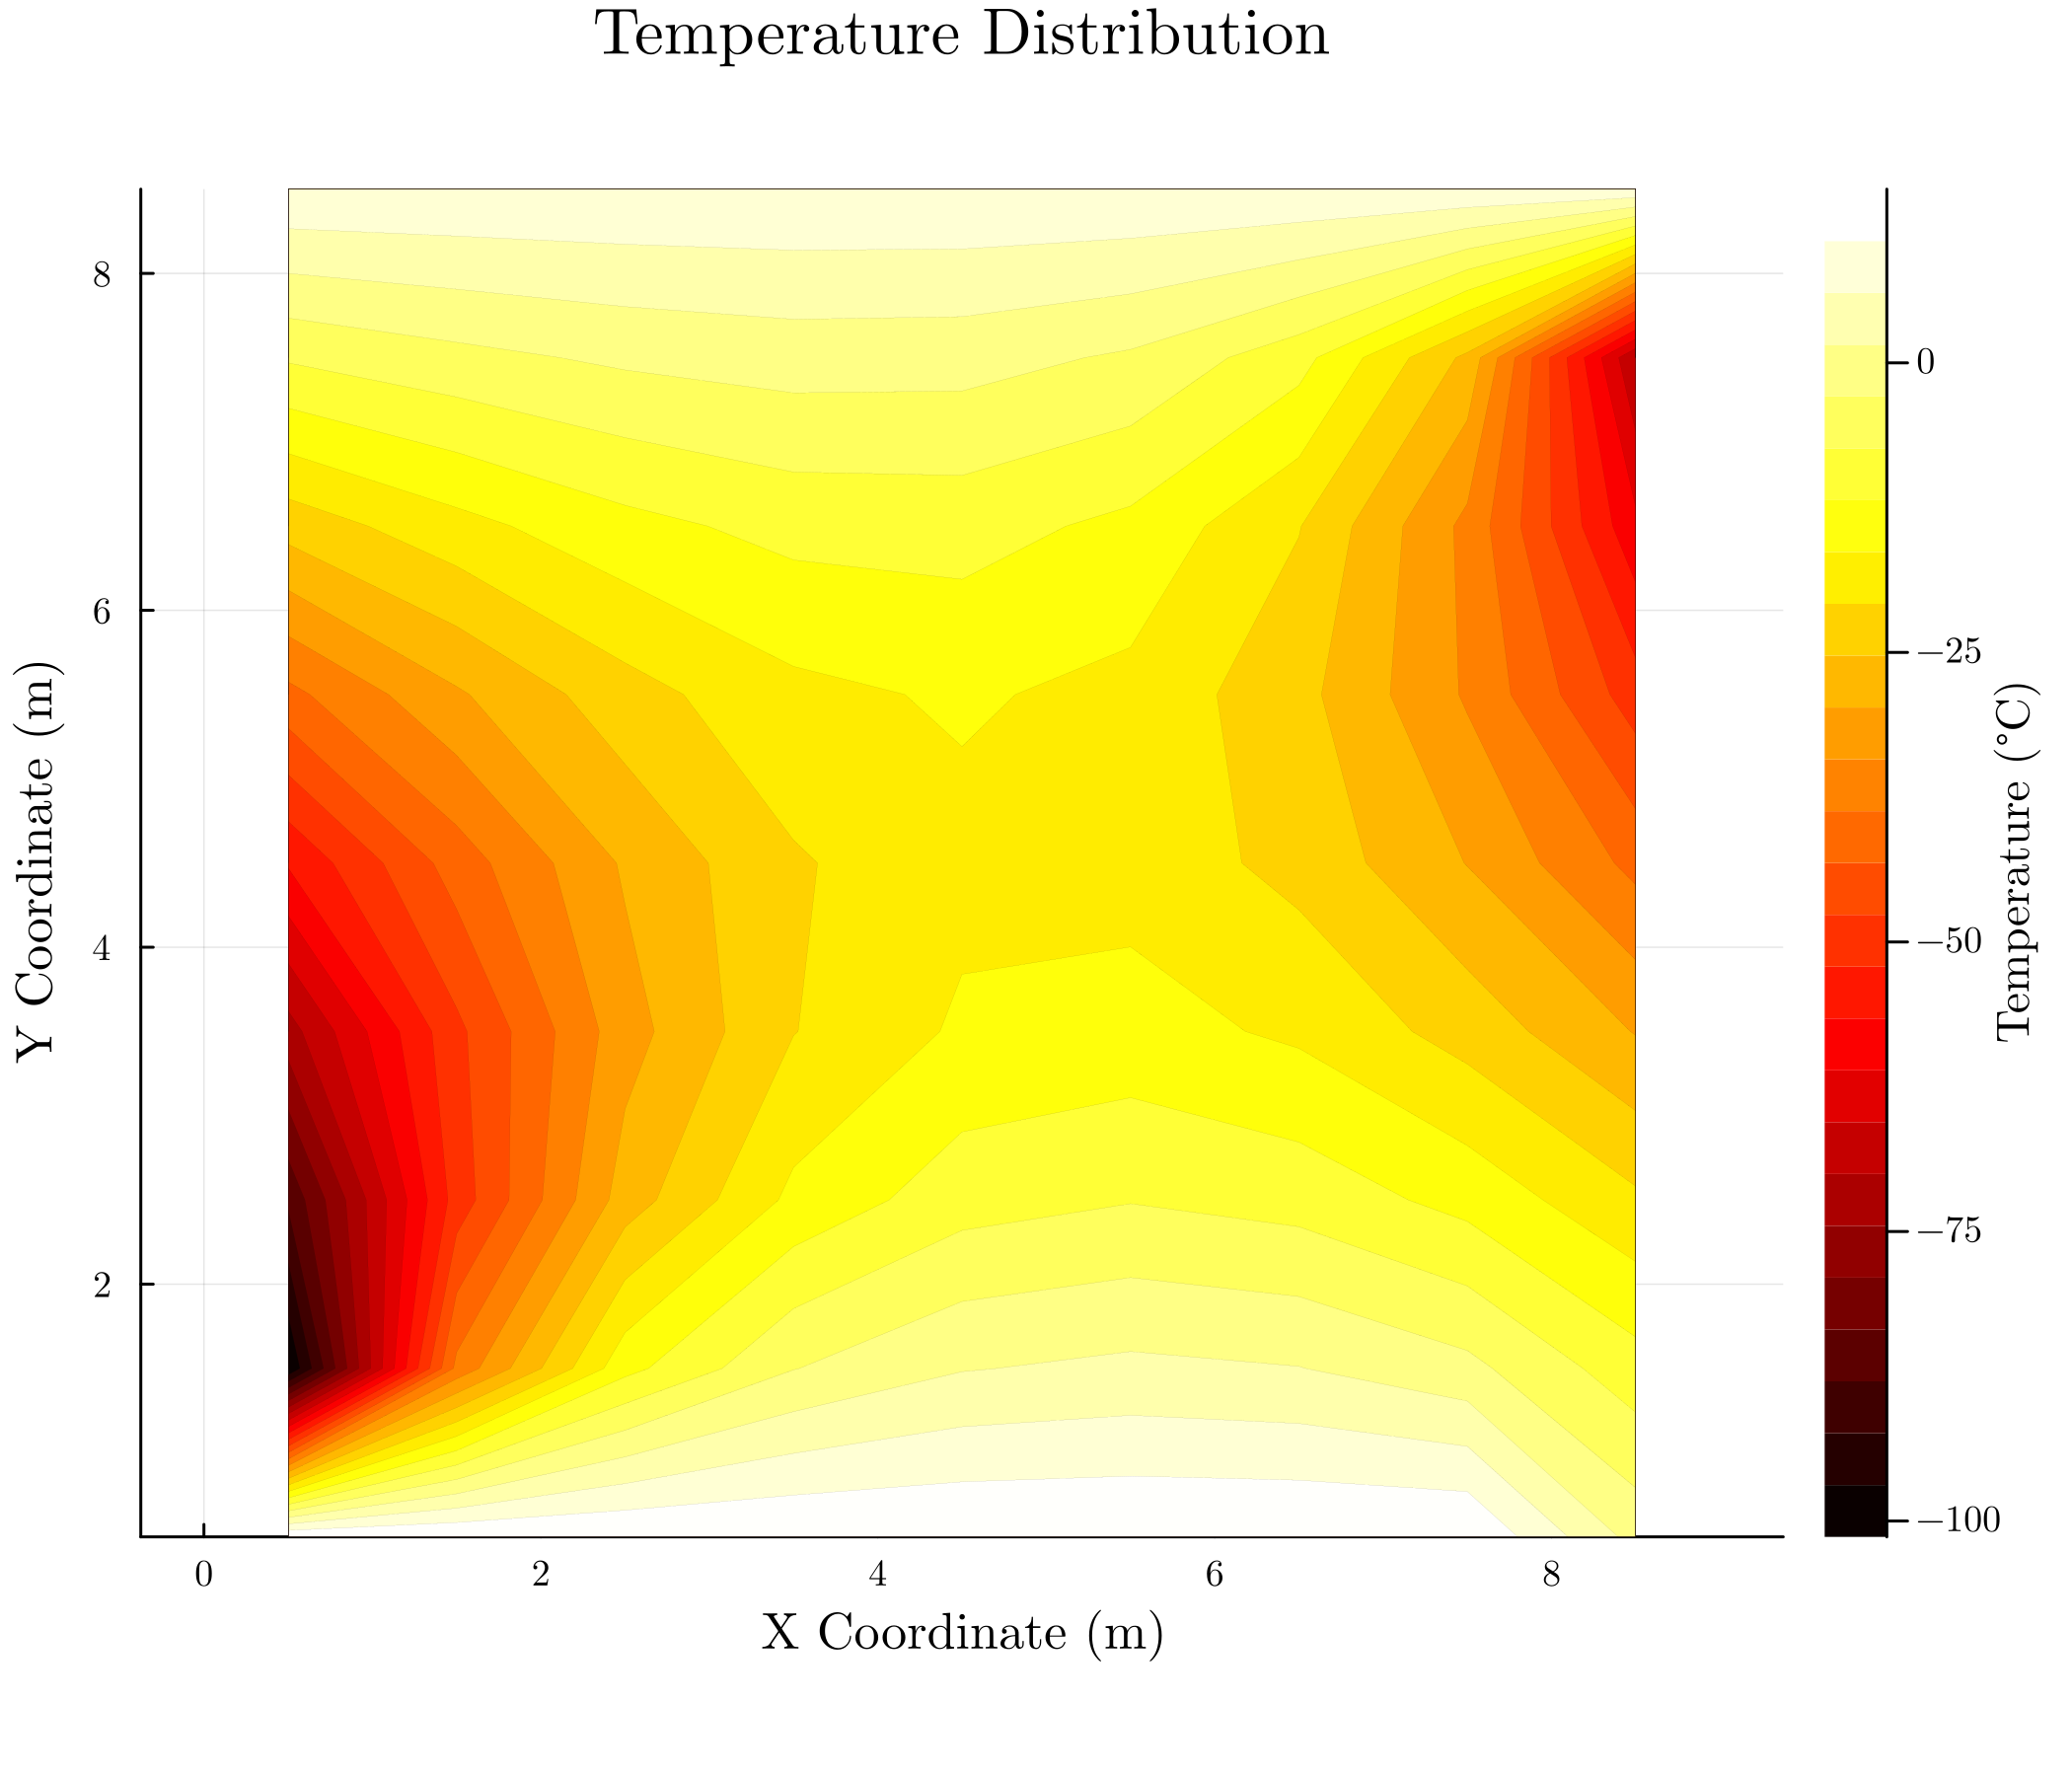
\includegraphics[width=.9\linewidth]{./plot2.png}
\end{center}
\subsection{Plot with n = 20}
\label{sec:org0e0ff05}

\begin{description}
\item[{delta\textsubscript{x}}] 0.1
\item[{delta\textsubscript{y}}] 0.1
\end{description}
\begin{center}
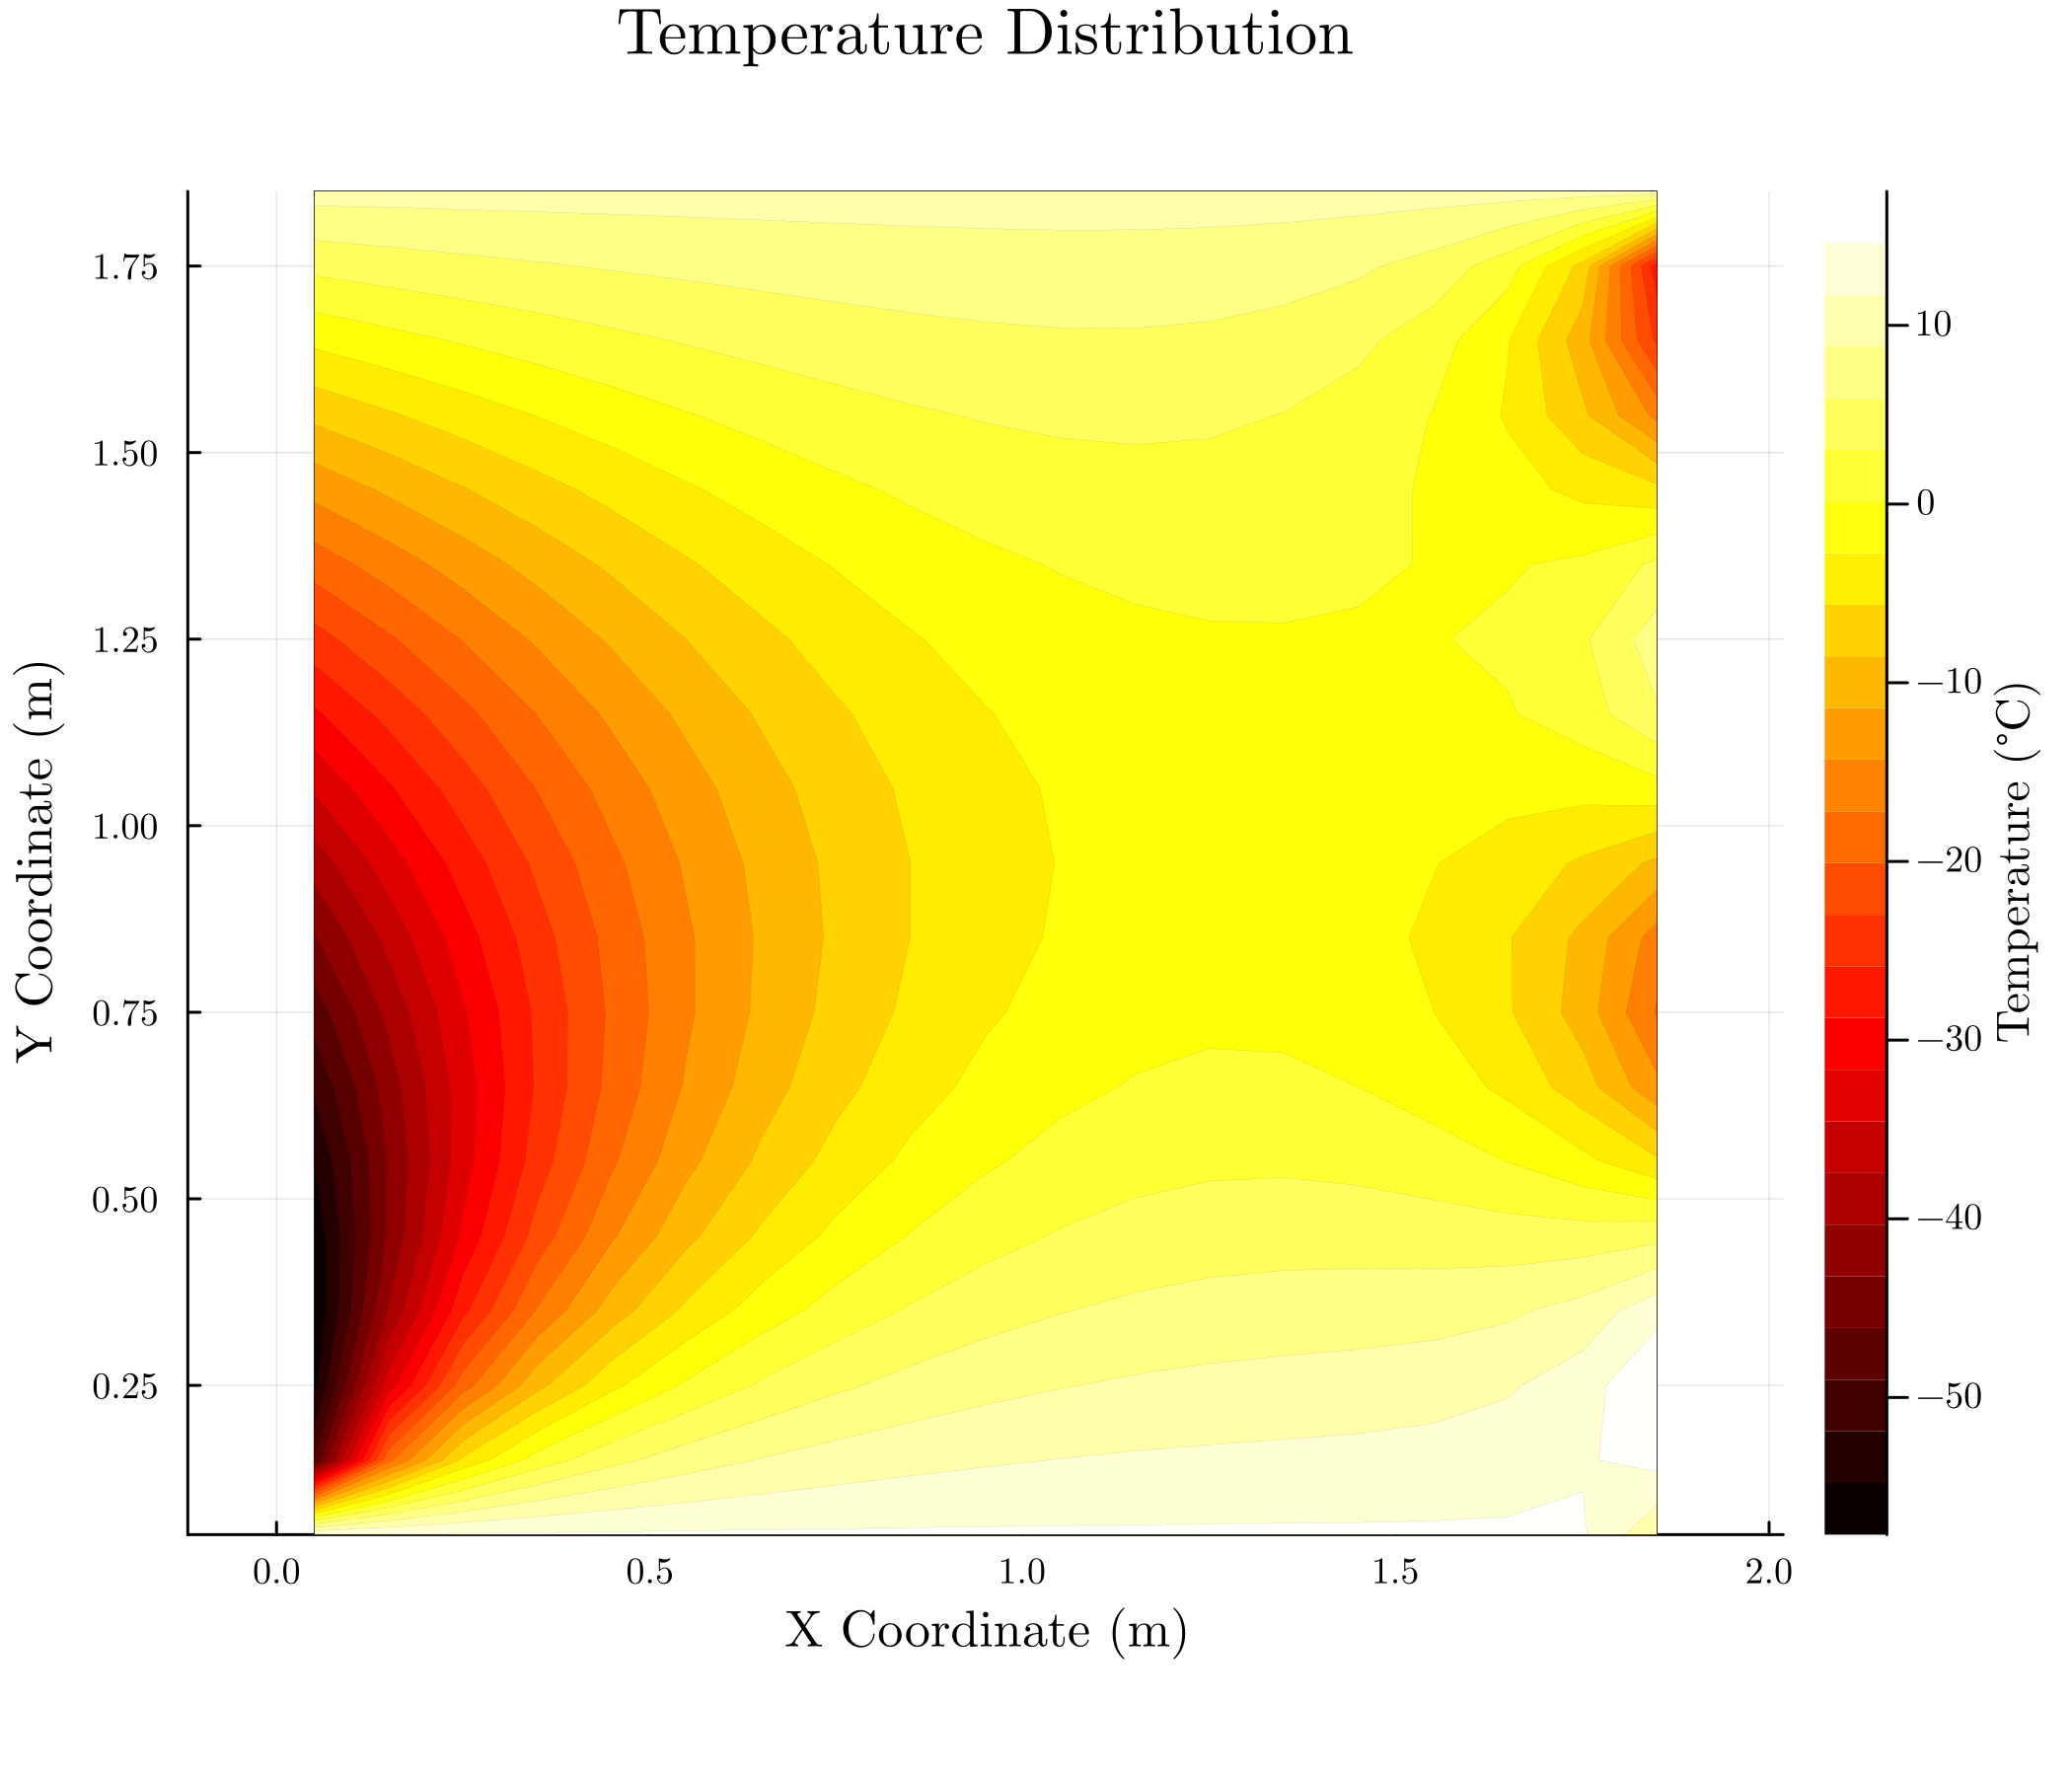
\includegraphics[width=.9\linewidth]{./plot1.png}
\end{center}
\subsection{n = 30}
\label{sec:orgae90f54}
\begin{description}
\item[{delta\textsubscript{x}}] 0.01
\item[{delta\textsubscript{y}}] 0.01
\end{description}
\begin{center}
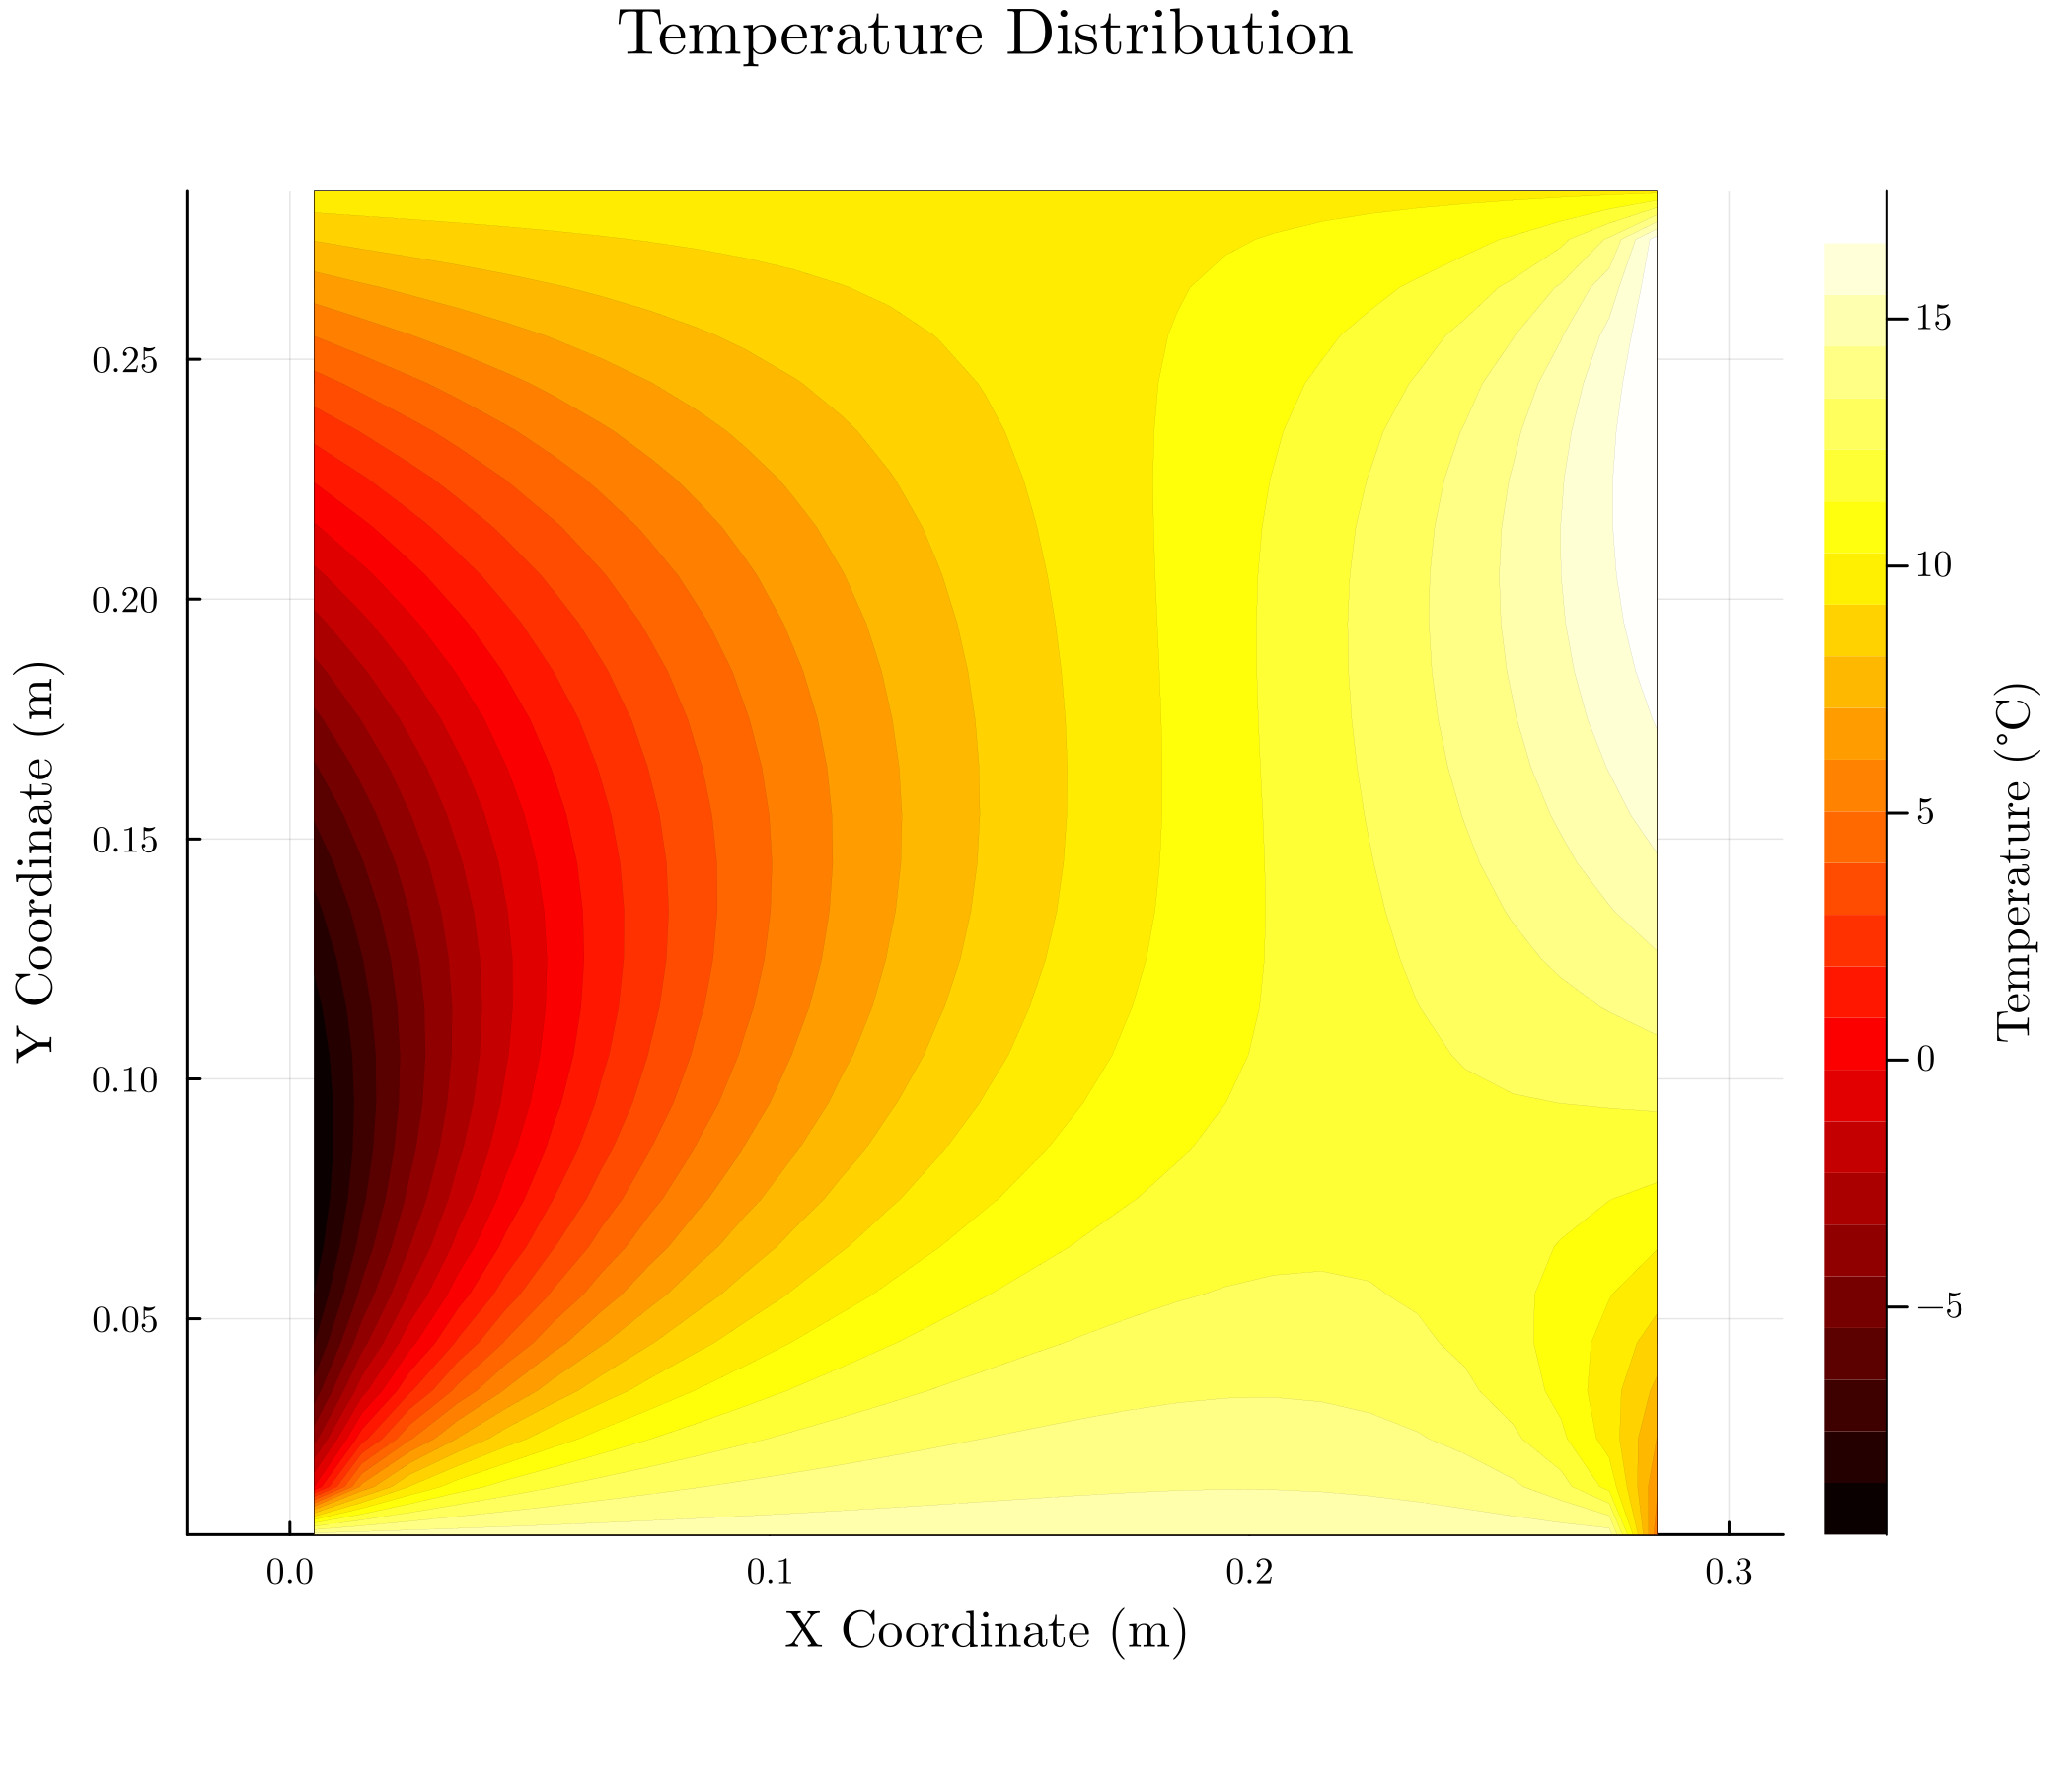
\includegraphics[width=.9\linewidth]{./plot4.png}
\end{center}

\begin{description}
\item[{delta\textsubscript{x}}] 1.0
\item[{delta\textsubscript{y}}] 1.0
\end{description}
\begin{center}
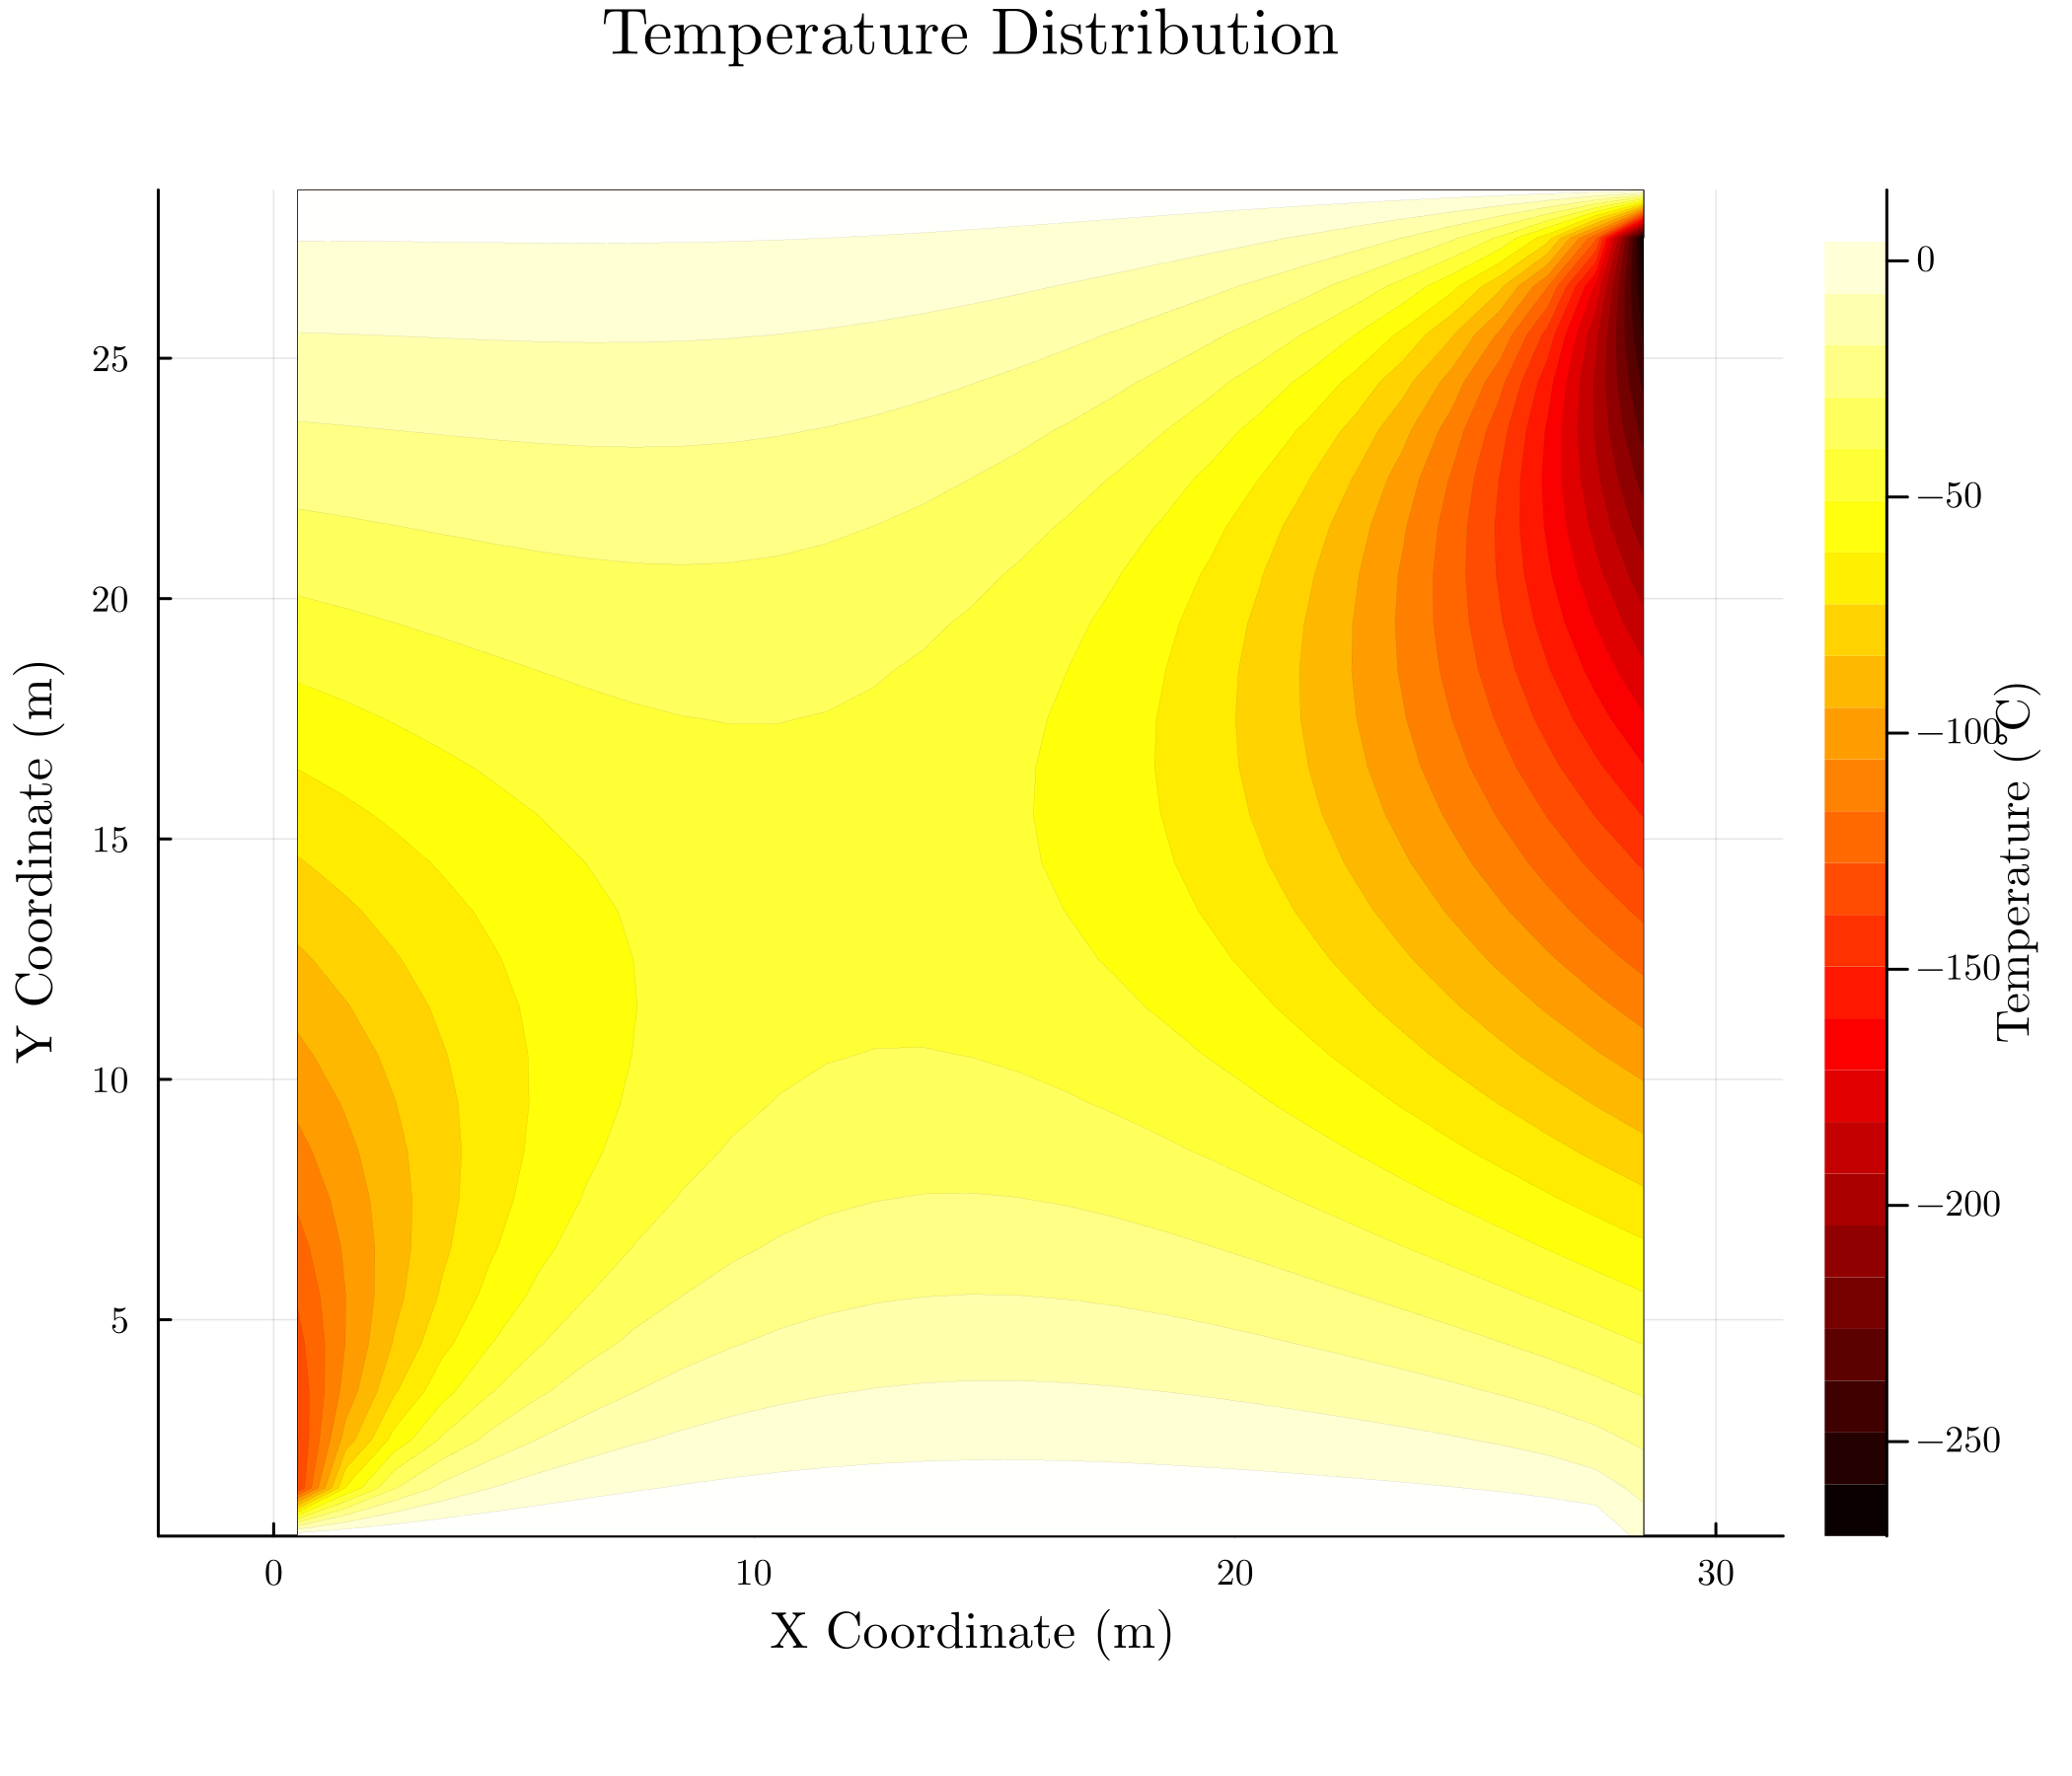
\includegraphics[width=.9\linewidth]{./plot5.png}
\end{center}
\subsection{Plot withn n = 40}
\label{sec:orgbb5db8c}

\begin{description}
\item[{delta\textsubscript{x}}] 0.01
\item[{delta\textsubscript{y}}] 0.01
\end{description}
\begin{center}
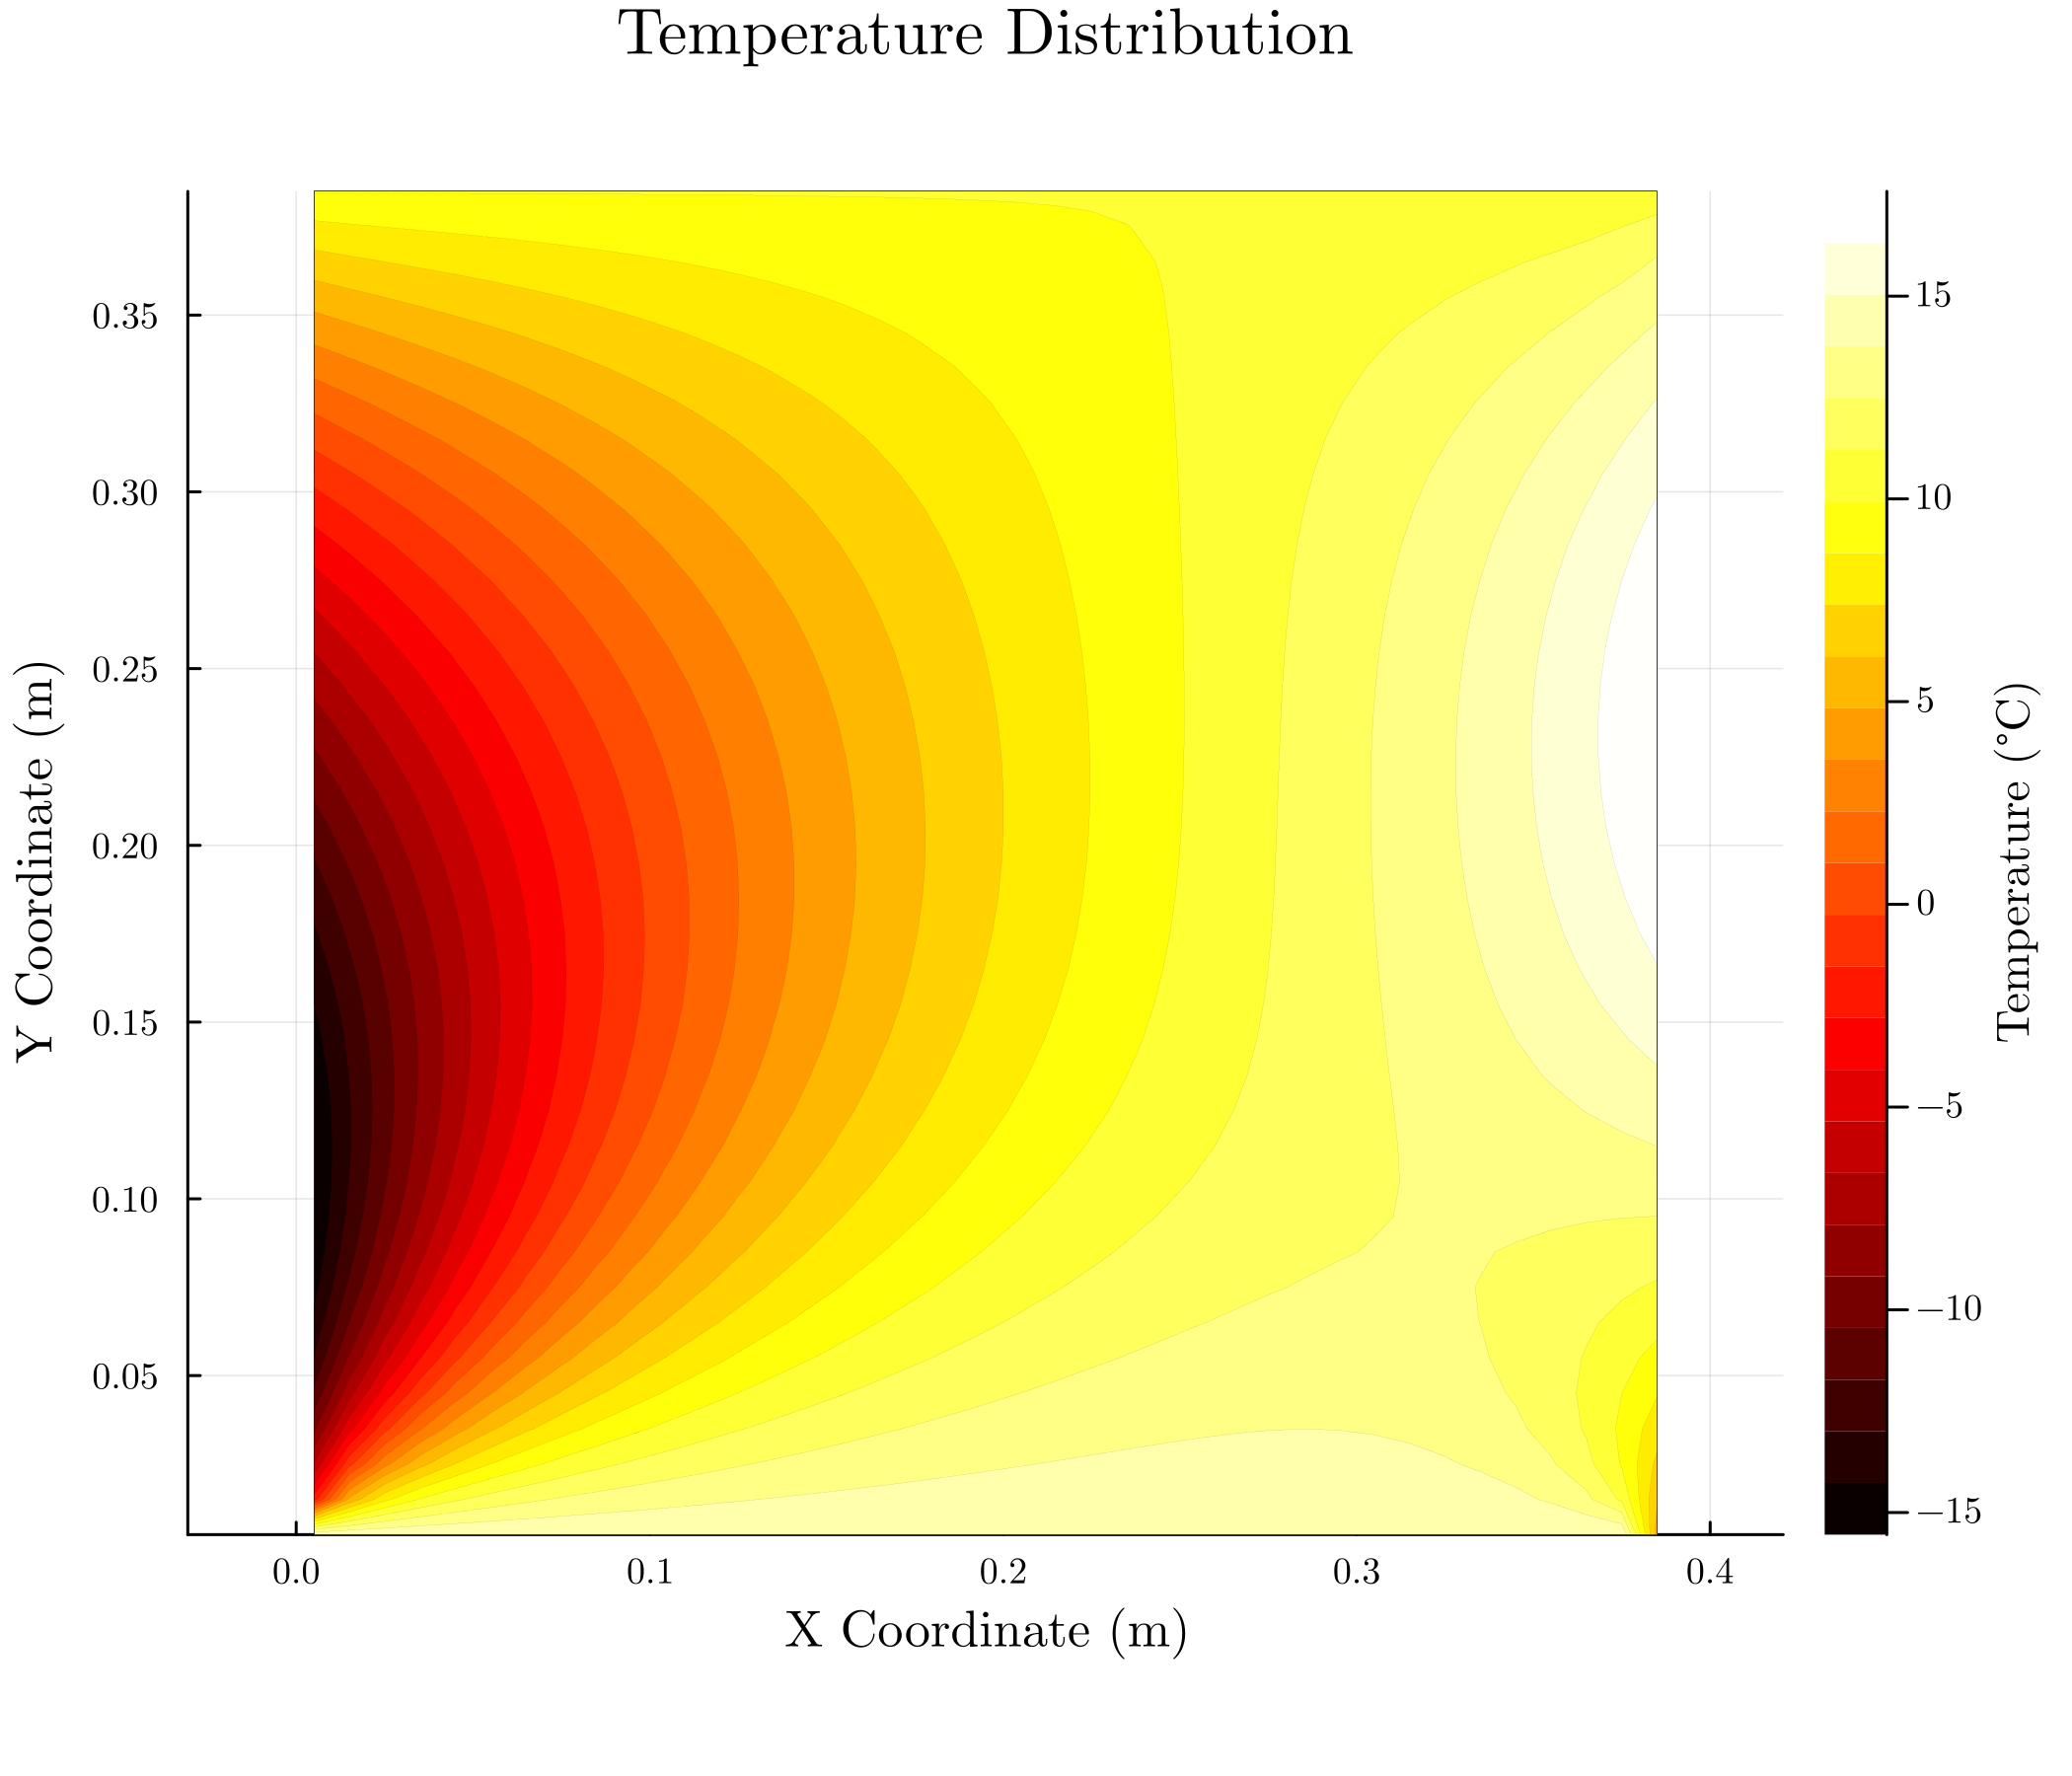
\includegraphics[width=.9\linewidth]{./plot3.png}
\end{center}
\section{Convergence History}
\label{sec:orgf722ce1}
This section contain the number of iteration required to achive desired convergence . the data is obtained and convergence history is plotted against logarithmic tolerane value

\begin{center}
\begin{tabular}{rr}
Tolerance & Iteration Number\\
\hline
0.1 & 7\\
0.01 & 14\\
0.001 & 81\\
0.0001 & 135\\
1e-05 & 187\\
1e-06 & 238\\
1e-07 & 289\\
1e-08 & 341\\
1e-09 & 392\\
1e-10 & 443\\
1e-11 & 495\\
\hline
\end{tabular}
\end{center}

\begin{center}
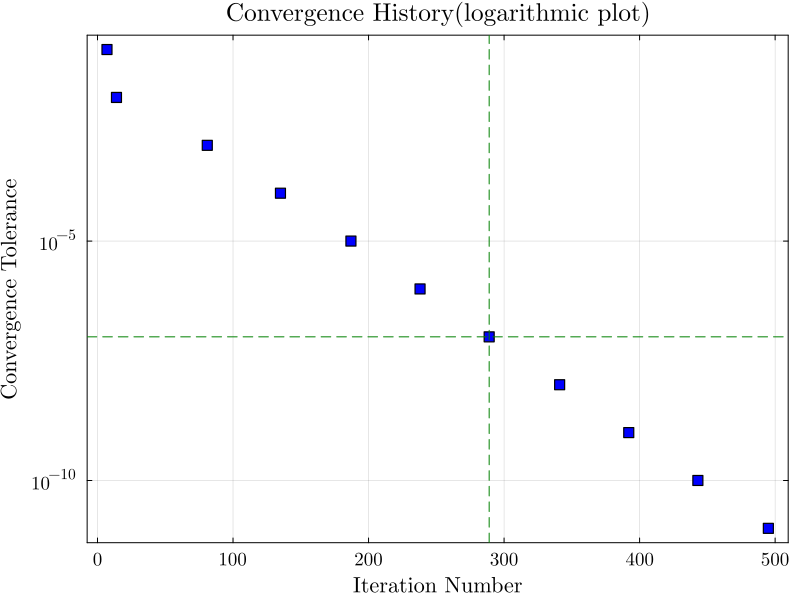
\includegraphics[width=.9\linewidth]{./converge_log.png}
\end{center}
\end{document}
